\documentclass[conference]{IEEEtran}
\usepackage[utf8]{inputenc}
\usepackage[T1]{fontenc}
\usepackage[brazil]{babel}
\usepackage{amsmath,amssymb}
\usepackage{graphicx}
\usepackage{booktabs}
\usepackage{url}

\begin{document}

\title{Identificação ARX e Controle Ótimo Discreto para Alocação Dinâmica em ITSA4}

\author{
\IEEEauthorblockN{Gabriel Negreiro Oliveira, Mateus Levi Morais Feitosa e Marcello Ryaj de Almeida Santos}
\IEEEauthorblockA{Instituto Tecnológico de Aeronáutica (ITA)\\
CMC-12: Sistemas de Controle Contínuos e Discretos}
}

\maketitle

\begin{abstract}
Este trabalho formula a alocação semanal de capital entre a ação da Itaúsa (ITSA4) e uma aplicação remunerada pelo CDI como um problema de controle em tempo discreto. A dinâmica do ativo é representada por um modelo ARX identificado a partir de dados de mercado e caracterizada por sua função de transferência de pulso $G(z)$, cujos polos determinam a estabilidade e a memória do sistema. Sobre o modelo aplicam-se três leis de controle sob um mesmo simulador: um controlador ótimo de horizonte unitário, também caracterizado como filtro discreto de primeira ordem $C(z)$; um controlador preditivo com restrição de caixa; e um regulador de volatilidade. Os hiperparâmetros são selecionados por busca em grade refinada pelo método de Nelder--Mead, e a avaliação emprega validação \emph{walk-forward} com re-identificação periódica, teste de significância por \emph{bootstrap} de blocos e análises de sensibilidade a custo de transação e a atraso de medida. Os resultados sustentam uma tese unificadora: a memória curta do sistema identificado (polo dominante de módulo $0{,}55$) explica por que o controle entrega o retorno do ativo com cerca de metade da volatilidade e um terço do rebaixamento máximo, por que o horizonte de predição ótimo é unitário e por que a predição multipasso não compensa atraso na malha. A vantagem em retorno sobre a estratégia passiva não é estatisticamente significativa; a contribuição robusta do arcabouço de controle é a redução de risco.
\end{abstract}

\begin{IEEEkeywords}
Identificação de sistemas, modelo ARX, função de transferência discreta, controle ótimo, controle preditivo, atraso, \emph{volatility targeting}.
\end{IEEEkeywords}

\section{Introdução}

A alocação de capital entre um ativo de risco e uma aplicação segura é um problema de decisão sequencial em tempo discreto: a cada semana escolhe-se a fração $u[k] \in [0,1]$ do capital mantida no ativo, permanecendo o restante em caixa remunerado pela taxa CDI. Neste trabalho o ativo é a ação da Itaúsa (ITSA4) e a decisão é semanal, o que define naturalmente um período de amostragem $T$ de uma semana e coloca o problema, desde a origem, no domínio em que operam os controladores digitais estudados em CMC-12.

A dificuldade central do problema é a baixa previsibilidade dos retornos financeiros. Sob a hipótese de mercados eficientes \cite{fama1970}, os preços incorporam rapidamente a informação disponível, de modo que a direção do retorno futuro comporta-se, em boa aproximação, como um processo imprevisível. Há, contudo, duas regularidades exploráveis. A primeira é estatística: a variância condicional dos retornos agrupa-se no tempo \cite{engle1982,bollerslev1986,cont2001}, o que torna a volatilidade prevísivel mesmo quando a direção não o é. A segunda é estrutural e constitui a pergunta de pesquisa deste trabalho: se um modelo dinâmico identificado a partir dos dados exibir polos afastados da origem, o sistema possui memória, e essa memória pode --- em princípio --- ser explorada por uma lei de controle baseada em predição. Quantificar essa memória e verificar até onde ela sustenta o controle é o objetivo do artigo.

A abordagem adotada percorre o ciclo completo de um projeto de controle. Identifica-se um modelo ARX para o retorno semanal da ITSA4 no arcabouço de erro de predição \cite{ljung1999}, com estimação por regressão de crista \cite{hoerl1970}. O modelo é caracterizado por sua função de transferência de pulso $G(z) = B(z)/A(z)$ \cite{astrom1997}: os polos informam estabilidade e memória, e a robustez de sua posição é examinada variando a regularização. Sobre o preditor aplicam-se três leis de controle: um controlador ótimo de horizonte unitário derivado de um custo quadrático, na linha da ponderação de esforço do regulador linear quadrático \cite{anderson1990}; um controlador preditivo baseado em modelo (MPC) com restrição de caixa \cite{camacho2007,mayne2000}; e um regulador de volatilidade \cite{moreira2017}, que dispensa a predição de retorno. Os hiperparâmetros do custo são selecionados por busca em grade seguida de refino pelo método de Nelder--Mead \cite{nelder1965}, com o ótimo da grade como estimativa inicial --- a mesma metodologia de projeto por otimização numérica empregada no curso. A avaliação usa janelas temporais disjuntas para seleção e teste, validação \emph{walk-forward} com re-identificação, significância por \emph{bootstrap} de blocos \cite{kunsch1989} e sensibilidade a custo de transação e a atraso de medida.

O trabalho traz três contribuições. Primeiro, a caracterização completa do sistema identificado e dos próprios elementos da malha no domínio $z$: além dos polos de $G(z)$, o controlador de horizonte unitário e o estimador de volatilidade são reduzidos a filtros de primeira ordem com polo, ganho DC e constante de tempo explícitos, o que dá interpretação dinâmica direta aos hiperparâmetros. Segundo, um protocolo experimental sem sobreposição entre janelas de seleção e de avaliação, verificado por uma suíte de testes que inclui a checagem automática de ausência de vazamento temporal. Terceiro, dois experimentos tipicamente ausentes em estudos aplicados de alocação: a degradação do desempenho com atraso de medida --- o análogo experimental do atraso de transporte estudado no curso --- e a seleção empírica do horizonte de predição, cujos resultados convergem para a mesma explicação estrutural dada pelos polos. A Seção~\ref{sec:teoria} apresenta a fundamentação; a Seção~\ref{sec:implementacao}, a implementação; a Seção~\ref{sec:resultados}, os resultados e sua discussão; a Seção~\ref{sec:conclusao} conclui.

\section{Fundamentação Teórica}\label{sec:teoria}

\subsection{Identificação do modelo ARX}

O retorno logarítmico semanal da ITSA4, denotado $r[k]$, é descrito por um preditor de um passo na forma
\begin{equation}
r[k+1] = \varphi[k]^{\top}\theta + e[k+1],
\label{eq:arx}
\end{equation}
em que $\varphi[k]$ reúne os regressores disponíveis no instante $k$ --- retornos defasados da própria ITSA4 (a parte autorregressiva), retornos de fatores exógenos e indicadores de volatilidade, tendência e nível de juros --- $\theta$ é o vetor de parâmetros e $e[k+1]$ é o erro de predição. Como a Itaúsa é uma \emph{holding} financeira dominada pelo Itaú, o conjunto exógeno é adaptado ao seu perfil: ITUB4, o índice Ibovespa, o câmbio USD/BRL, o ETF de Brasil em dólar (EWZ, aproximação do fluxo estrangeiro), o índice VIX e o nível do CDI. Os regressores são fortemente correlacionados entre si, o que degrada a variância do estimador de mínimos quadrados; por isso adota-se a regressão de crista \cite{hoerl1970},
\begin{equation}
\hat{\theta} = \arg\min_{\theta}\ \sum_k w[k]\bigl(r[k+1]-\varphi[k]^{\top}\theta\bigr)^2 + \alpha\lVert\theta\rVert_2^2,
\label{eq:ridge}
\end{equation}
com regularização $\alpha>0$ e pesos temporais $w[k]$ que privilegiam o passado recente. A penalização $\ell_2$ introduz viés de encolhimento nos coeficientes; a consequência dessa escolha sobre a posição dos polos é examinada empiricamente na Seção~\ref{sec:res-tf}.

\subsection{Função de transferência de pulso e estabilidade}

A parte linear do modelo \eqref{eq:arx} define um sistema em tempo discreto cuja função de transferência de pulso é $G(z) = B(z)/A(z)$ \cite{astrom1997}, com denominador
\begin{equation}
A(z) = z^{4} - a_1 z^{3} - a_2 z^{2} - a_3 z - a_4
\end{equation}
formado pelos quatro coeficientes autorregressivos identificados, e numeradores $B_i(z)$ associados a cada entrada exógena. O sistema é assintoticamente estável se, e somente se, todos os polos satisfazem $|z_i| < 1$, condição que é o análogo discreto do semiplano esquerdo do plano $s$ sob o mapeamento $z = e^{sT}$. Os polos carregam, além da estabilidade, a informação de memória: a resposta ao impulso de cada modo decai como $|z_i|^k$, de modo que o módulo do polo dominante fixa a escala de tempo em que informação passada permanece relevante. Os regressores não lineares (volatilidades, tendências, volume e níveis) não compõem uma descrição LTI e ficam fora da decomposição; os polos extraídos descrevem, portanto, a dinâmica linear condicional do sistema, e não o modelo completo --- uma limitação declarada da análise.

\subsection{A alocação como problema de controle}

É preciso explicitar qual é a planta. A ação de controle não altera a dinâmica do preço, pois uma carteira pequena não move o mercado; o ARX atua como modelo de perturbação mensurável e preditor, não como planta realimentada. A planta propriamente dita é a dinâmica do capital,
\begin{equation}
C[k+1] = C[k]\bigl[1 + u[k]\,r[k+1] + (1-u[k])\,r_{\mathrm{cdi}}[k+1] - c\,|\Delta u[k]|\bigr],
\label{eq:planta}
\end{equation}
em que $\Delta u[k] = u[k]-u[k-1]$ e $c$ é o custo proporcional de transação. O estado relevante é o par $(C[k],\,u[k-1])$, a entrada de controle é $u[k]$ e os retornos são entradas exógenas estocásticas. A malha fecha-se pela medição: a cada semana medem-se os retornos realizados e a volatilidade, o preditor é atualizado e a lei de controle recalcula $u[k]$ a partir de $u[k-1]$ e das predições. Trata-se de realimentação sobre o estado da carteira com ação antecipatória das predições, estrutura usual em controle preditivo com perturbação medida \cite{camacho2007}. Cabe registrar o que essa estrutura implica: conceitos de malha aberta LTI, como margens de ganho e de fase, não se aplicam aqui, pois não existe função de transferência de malha cruzando $-180^{\circ}$; o papel de ``margem'' é exercido, neste trabalho, pela análise experimental de tolerância a atraso da Seção~\ref{sec:res-atraso}.

\subsection{Controle ótimo de horizonte unitário e sua leitura em frequência}\label{sec:teoria-h1}

O controlador de horizonte unitário minimiza, a cada semana, o custo quadrático
\begin{equation}
J[k] = -\hat{r}[k+1]\,u[k] + \lambda\,u[k]^2 + \rho\,(u[k]-u[k-1])^2,
\label{eq:custoh1}
\end{equation}
em que $\hat{r}[k+1]$ é o retorno previsto pelo ARX, $\lambda$ penaliza o tamanho da posição --- o esforço de controle, na acepção do regulador linear quadrático \cite{anderson1990} --- e $\rho$ penaliza a variação da posição, substituto quadrático suave do custo real $c\,|\Delta u|$ de \eqref{eq:planta}. O mínimo irrestrito tem forma fechada,
\begin{equation}
u^{*}[k] = \frac{\hat{r}[k+1]+2\rho\,u[k-1]}{2(\lambda+\rho)},
\label{eq:leih1}
\end{equation}
saturada em seguida ao intervalo $[0,1]$.

Fora da saturação, \eqref{eq:leih1} é a recursão linear $u[k] = a\,u[k-1] + b\,\hat{r}[k+1]$ com $a = \rho/(\lambda+\rho)$ e $b = 1/(2(\lambda+\rho))$, ou seja, o controlador é um filtro passa-baixas discreto de primeira ordem,
\begin{equation}
C(z) = \frac{U(z)}{\hat{R}(z)} = \frac{b\,z}{z-a},
\label{eq:cz}
\end{equation}
estável para quaisquer $\lambda,\rho > 0$ (o polo $a$ pertence a $[0,1)$), com ganho DC $b/(1-a) = 1/(2\lambda)$ e constante de tempo $-T/\ln a$. Essa leitura conecta os hiperparâmetros do custo diretamente à resposta em frequência: $\rho$ posiciona o polo e, com ele, a banda passante do controlador; $\lambda$ fixa o ganho estático, de modo que em regime permanente $u_{\infty} = \hat{r}/(2\lambda)$, saturando em $1$ para predições sustentadas $\hat{r} \ge 2\lambda$. A equivalência entre a lei implementada e o filtro \eqref{eq:cz} é verificada numericamente pela suíte de testes do projeto.

\subsection{Controle preditivo baseado em modelo}

A generalização natural de \eqref{eq:custoh1} considera um horizonte de predição $H$. Escrevendo a parte autorregressiva do ARX como um registro de deslocamento de estados, predizem-se $\hat{r}[k+1],\dots,\hat{r}[k+H]$ por recursão --- as entradas exógenas são mantidas congeladas, pois não há modelo para sua evolução --- e minimiza-se
\begin{equation}
J = \sum_{j=0}^{H-1}\Bigl[-\hat{r}[k+j+1]\,u[k+j] + \lambda\,u[k+j]^2 + \rho\,\Delta u[k+j]^2\Bigr]
\label{eq:custompc}
\end{equation}
sujeito a $0 \le u[k+j] \le 1$, aplicando-se apenas o primeiro movimento $u[k]$ e repetindo o procedimento na semana seguinte (horizonte deslizante) \cite{camacho2007}. O problema é de programação quadrática convexa com restrições de caixa \cite{boyd2004}, resolvido numericamente a cada passo; propriedades gerais de estabilidade e otimalidade do MPC com restrições são estabelecidas em \cite{mayne2000}. Note-se a ligação estrutural com a análise de $G(z)$: o valor do horizonte $H$ só agrega informação se a predição multipasso tiver conteúdo, e o decaimento $|z_i|^k$ dos modos impõe um teto a esse conteúdo. Essa previsão teórica é testada empiricamente na Seção~\ref{sec:res-horizonte}.

\subsection{Regulador de volatilidade e filtragem da medida}

Como alternativa que não depende da predição de retorno, considera-se o regulador de volatilidade \cite{moreira2017}. A variância condicional é estimada pela média móvel exponencialmente ponderada da metodologia RiskMetrics \cite{riskmetrics1996},
\begin{equation}
\hat{\sigma}^2[k] = \lambda_v\,\hat{\sigma}^2[k-1] + (1-\lambda_v)\,r^2[k],
\label{eq:ewma}
\end{equation}
com fator de decaimento $\lambda_v = 0{,}94$, e a exposição é regulada para manter a volatilidade da carteira próxima de um alvo $\sigma^{*}$:
\begin{equation}
u[k] = \mathrm{sat}_{[0,1]}\!\left(\frac{\sigma^{*}}{\hat{\sigma}[k]}\right).
\end{equation}
A recursão \eqref{eq:ewma} merece a mesma leitura em frequência dada ao controlador: trata-se de um filtro passa-baixas de primeira ordem com função de transferência $F(z) = (1-\lambda_v)\,z/(z-\lambda_v)$, polo em $\lambda_v$, ganho DC unitário e constante de tempo $-T/\ln\lambda_v \approx 16$ semanas. O estimador de volatilidade é, portanto, um caso direto de filtragem de medida ruidosa por sistema de primeira ordem, como estudado no curso: o quadrado do retorno é uma medida instantânea extremamente ruidosa da variância, e o filtro extrai sua componente lenta ao custo de atraso de acompanhamento. Uma variante do regulador incorpora um viés multiplicativo limitado, função do sinal da predição do ARX, permitindo medir o valor marginal do preditor sobre uma base que não depende dele.

\subsection{Efeito de atraso na malha}\label{sec:teoria-atraso}

Em sistemas amostrados, a discretização introduz por si só um atraso médio de $T/2$, e atrasos adicionais de medida ou processamento consomem margem de estabilidade, pois a fase perdida cresce linearmente com a frequência ($\angle e^{-\tau j\omega} = -\tau\omega$). Na malha de alocação não há margem de fase a medir, mas o mecanismo de dano é o mesmo e pode ser quantificado diretamente: se a predição $\hat{r}$ e as medidas chegarem ao controlador com $n$ semanas de atraso, a ação $u[k]$ passa a responder a um estado defasado do mercado. O experimento correspondente desloca predições e regressores em $n \in \{0,1,2\}$ semanas e mede a degradação do desempenho, oferecendo um análogo experimental, em malha estocástica, do efeito do atraso de transporte sobre sistemas realimentados.

\subsection{Seleção de hiperparâmetros por otimização numérica}\label{sec:teoria-otim}

Os hiperparâmetros $(\lambda,\rho)$ não admitem solução analítica, pois o desempenho depende da trajetória simulada da carteira com saturação e custos. Adota-se a metodologia de projeto por otimização numérica empregada no curso: define-se a função de custo $J(\mathbf{x}) = -S_{\mathrm{val}}(\lambda,\rho)$, em que $S_{\mathrm{val}}$ é o índice de Sharpe da carteira simulada na janela de validação e $\mathbf{x} = [\log_{10}\lambda,\ \log_{10}\rho]^{\top}$, e minimiza-se $J$ pelo método de Nelder--Mead \cite{nelder1965}, com estimativa inicial dada pelo ótimo de uma busca em grade. A parametrização logarítmica condiciona o problema, já que os valores plausíveis varrem quatro décadas. Como o Nelder--Mead é irrestrito e a superfície de custo de dados financeiros pode empurrar parâmetros a valores degenerados (em particular $\rho \to 0$, que reduziria o controlador a ganho estático), o custo é definido como infinito fora da faixa coberta pela grade, confinando o refino à região de confiança do projetista. O horizonte $H$ do MPC, por ser inteiro, é selecionado por varredura direta.

\subsection{Avaliação e significância estatística}

O desempenho ajustado ao risco é medido pelo índice de Sharpe \cite{sharpe1994} sobre o excesso de retorno em relação ao CDI, anualizado por $\sqrt{P}$ com $P=52$. Para que a seleção de hiperparâmetros não contamine a avaliação, as janelas são disjuntas: identificação inicial no treino, escolha de $(\lambda,\rho,H)$ na validação e avaliação em duas frentes independentes --- um conjunto de teste posterior a todas as escolhas e uma validação \emph{walk-forward} que re-identifica o modelo periodicamente usando apenas o passado. A significância é apurada por \emph{bootstrap} de blocos móveis \cite{kunsch1989}, que preserva a autocorrelação dos retornos, produzindo intervalos de confiança para o Sharpe e um valor-$p$ para a hipótese de não superar o \emph{benchmark} passivo. A qualidade do preditor, premissa de todo o arcabouço, é medida separadamente por RMSE, acurácia direcional e correlação, sempre em comparação com o preditor nulo $\hat{r} = 0$, que é o previsor ótimo sob a hipótese de mercado eficiente.

\section{Implementação}\label{sec:implementacao}

\subsection{Arquitetura}

A implementação, em Python, organiza-se em módulos de responsabilidade única --- configuração, dados, regressores, identificação, estratégias, simulação, métricas, função de transferência e geração de saídas --- coordenados por um orquestrador que apenas encadeia as fases. Toda a parametrização do estudo (datas das janelas, ativos, grades, custos) reside em uma única estrutura imutável, o que estabelece fonte única de verdade e impede alteração acidental em tempo de execução. A identificação usa a biblioteca scikit-learn \cite{pedregosa2011}, com padronização ajustada apenas no treino; a otimização (Nelder--Mead na seleção de hiperparâmetros e o programa quadrático do MPC) usa a biblioteca SciPy \cite{virtanen2020}. As bibliotecas resolvem componentes bem delimitados; o simulador, as leis de controle, a análise em $z$, o \emph{walk-forward} e o \emph{bootstrap} são implementações próprias.

\subsection{Contrato único de simulação}

As estratégias compartilham um contrato: dada a informação disponível na semana $k$ --- predição, volatilidade estimada e posição anterior ---, cada uma devolve $u[k]$, e um único simulador aplica a dinâmica \eqref{eq:planta} a todas. Essa decisão garante, por construção, comparação justa: qualquer diferença de desempenho decorre da lei de controle, nunca de diferenças na contabilidade de custos ou de caixa. Na validação \emph{walk-forward}, o MPC é instanciado em variante com modelo variante no tempo, que usa em cada semana o modelo re-identificado vigente naquela data, treinado somente com o passado.

\subsection{Separação temporal}

As janelas são: treino de 2022 a 2023 para a identificação inicial; validação em 2024 para a escolha de $(\lambda,\rho,H)$; re-treino de 2023 até dezembro de 2025, com folga antes do teste para que o último rótulo de treino não se sobreponha à janela seguinte; teste no primeiro semestre de 2026; e \emph{walk-forward} de 2025 em diante, com re-identificação a cada quatro semanas em janela expansível. Nenhuma janela de seleção sobrepõe janela de avaliação, de modo que tanto o teste quanto o \emph{walk-forward} são integralmente fora da amostra, inclusive quanto aos hiperparâmetros.

\subsection{Verificação e reprodutibilidade}

Os dados brutos são salvos em \emph{snapshot} na primeira execução e recarregados nas seguintes, tornando os resultados reprodutíveis mesmo com revisões das fontes públicas. Uma suíte de verificação offline confere as peças centrais com dados sintéticos: a equivalência entre o resolvedor do programa quadrático e busca exaustiva; a coincidência entre o MPC de horizonte unitário, a lei analítica \eqref{eq:leih1} e o filtro \eqref{eq:cz}; a fórmula da banda passante de $-3$~dB dos filtros de primeira ordem; a ausência de vazamento temporal no \emph{walk-forward}, checada por um treinador instrumentado que acusa qualquer predição sobre dados de treino; o confinamento do refino de Nelder--Mead à faixa da grade; e a degradação de desempenho sob atraso com predição perfeita, caso em que o resultado é conhecido por construção.

\section{Resultados e Discussão}\label{sec:resultados}

Esta seção sustenta a tese de que a estrutura dinâmica identificada explica o comportamento de todas as leis de controle. O argumento parte da qualidade do preditor, passa pela caracterização em $z$ do sistema e do controlador e culmina nos experimentos de desempenho, horizonte, custo e atraso, que convergem para a mesma explicação.

\subsection{Qualidade do preditor identificado}

A Tabela~\ref{tab:previsor} compara o ARX com o preditor nulo. No \emph{walk-forward}, o modelo re-identificado supera o nulo em RMSE ($0{,}0301$ contra $0{,}0312$), acerta a direção do retorno em $57{,}7\%$ das semanas e apresenta correlação de $0{,}30$ com o retorno realizado --- evidência de estrutura explorável, ainda que modesta. No conjunto de teste, o quadro é mais matizado: o RMSE do ARX é ligeiramente pior que o do nulo, com acurácia direcional de $50\%$, mas a correlação de $0{,}17$ permanece positiva. A leitura conjunta indica que o valor do preditor para alocação não está na magnitude prevista, e sim no ordenamento das semanas: uma predição correlacionada com o realizado desloca a exposição para as semanas certas mesmo errando o tamanho do retorno. Essa distinção explica como, na Seção~\ref{sec:res-teste}, um preditor com RMSE inferior ao nulo sustenta um controlador com desempenho muito superior ao passivo --- e recomenda cautela contra julgar preditores de alocação apenas por erro quadrático.

\begin{table}[!t]
\centering
\caption{Qualidade do preditor contra o preditor nulo $\hat{r}=0$.}
\label{tab:previsor}
\begin{tabular}{lccc}
\toprule
Preditor & RMSE & Acur. direc. & Correl. \\
\midrule
ARX (teste)            & $0{,}0398$ & $50{,}0\%$ & $0{,}17$ \\
Nulo (teste)           & $0{,}0396$ & ---        & ---      \\
ARX (\emph{walk-f.})   & $0{,}0301$ & $57{,}7\%$ & $0{,}30$ \\
Nulo (\emph{walk-f.})  & $0{,}0312$ & ---        & ---      \\
\bottomrule
\end{tabular}
\end{table}

Os coeficientes identificados são economicamente coerentes com o perfil da Itaúsa: os maiores pesos padronizados recaem sobre o retorno contemporâneo do EWZ ($+0{,}027$) e do Ibovespa ($-0{,}025$), seguidos do EWZ defasado ($+0{,}011$), do câmbio e do Itaú. O peso apreciável de um regressor defasado é o primeiro indício de memória: parte do retorno da semana seguinte relaciona-se com informação já observada.

\subsection{Análise por função de transferência}\label{sec:res-tf}

Os quatro polos de $G(z)$ situam-se no interior do círculo unitário (Fig.~\ref{fig:polos}): um par complexo dominante em $0{,}19 \pm 0{,}51j$, de módulo $0{,}55$, e um par secundário de módulo $0{,}25$. O sistema é estável e possui memória curta, porém não nula: a envoltória da resposta ao impulso do modo dominante decai como $0{,}55^k$, o que dá profundidade efetiva da ordem de $1/(1-0{,}55) \approx 2$ semanas. O ângulo de aproximadamente $70^{\circ}$ do par dominante corresponde a um modo oscilatório com período próximo de cinco semanas, coerente com os coeficientes autorregressivos negativos estimados (reversão à média). Duas qualificações disciplinam a leitura. Primeiro, o módulo do polo majora a persistência dos modos, mas não mede a fração do retorno explicada pela dinâmica linear --- essa fração é pequena, como a Tabela~\ref{tab:previsor} mostra. Segundo, os polos provêm de coeficientes encolhidos pela regularização; para verificar se sua posição é artefato do $\alpha$ escolhido, repetiu-se a identificação com $\alpha \in \{0{,}1;\,0{,}3;\,1;\,3;\,10\}$: o raio espectral variou apenas de $0{,}52$ a $0{,}56$, sempre estável. A memória curta é, portanto, propriedade robusta dos dados, e não da regularização. A Fig.~\ref{fig:freqarx} complementa com a resposta em frequência por entrada exógena.

\begin{figure}[!t]
\centering
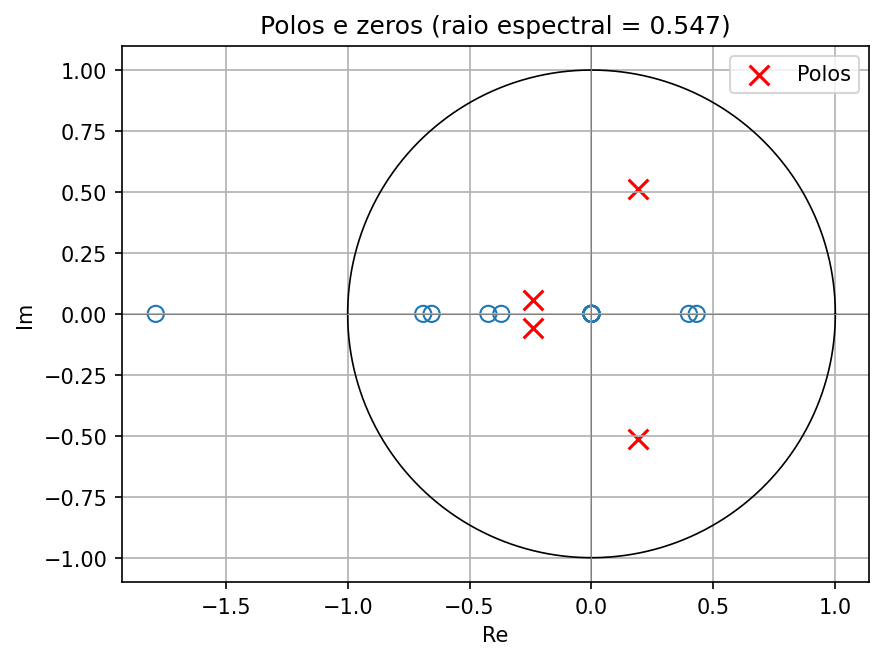
\includegraphics[width=0.82\columnwidth]{figuras/mapa_polos_zeros_arx.png}
\caption{Mapa de polos e zeros do ARX identificado. Todos os polos estão no interior do círculo unitário; raio espectral de $0{,}547$, estável para $\alpha$ variando duas décadas.}
\label{fig:polos}
\end{figure}

\begin{figure}[!t]
\centering
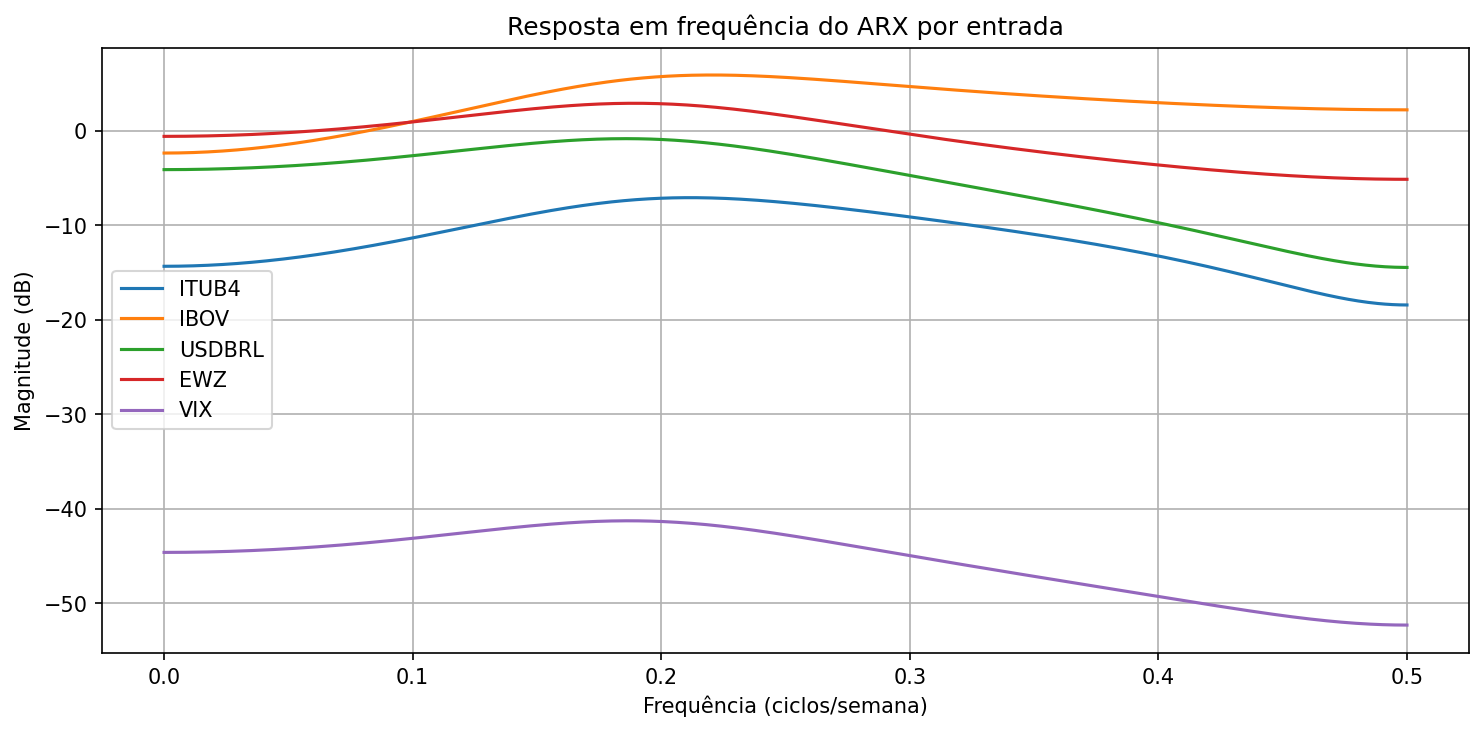
\includegraphics[width=\columnwidth]{figuras/resposta_frequencia_arx.png}
\caption{Resposta em frequência $|G_i(e^{j\omega})|$ do ARX por entrada exógena.}
\label{fig:freqarx}
\end{figure}

\subsection{Hiperparâmetros e o controlador como filtro}\label{sec:res-filtro}

A busca em grade na validação de 2024 indicou $\lambda = 0{,}01$ e $\rho = 0{,}001$, com Sharpe de validação $-0{,}93$; o refino por Nelder--Mead melhorou o custo para $-0{,}88$, convergindo para $\lambda = 0{,}0085$ e $\rho = 0{,}0010$, este na borda inferior da faixa admissível. Dois fatos merecem interpretação. O primeiro é o sinal negativo: 2024 foi um ano adverso para a ITSA4, no qual nenhuma combinação de hiperparâmetros bateu o CDI; a seleção opera, legitimamente, escolhendo a lei menos vulnerável em cenário desfavorável, e o valor absoluto do Sharpe de validação não prediz o desempenho futuro --- apenas ordena as alternativas. O segundo é a pressão do otimizador contra $\rho$: sem a restrição à faixa da grade, o refino levaria $\rho \to 0$, degenerando o controlador em ganho estático. O dado sugere que, nesta planta e nesta janela, a suavização por $\rho$ pouco contribui, e que o amortecimento útil da lei vem majoritariamente de $\lambda$, que limita o tamanho da posição.

Com os valores selecionados, o controlador \eqref{eq:cz} tem polo $a = 0{,}105$, constante de tempo de $0{,}44$ semana e ganho DC de $58{,}6$ --- em regime, satura a exposição para predições sustentadas acima de $2\lambda \approx 1{,}7\%$ na semana. É um filtro fraco: a atenuação máxima, na frequência de Nyquist, é de apenas $1{,}9$~dB, de modo que o controlador jamais atinge o corte convencional de $-3$~dB (Fig.~\ref{fig:ctrl}). O contraste com o estimador de volatilidade é instrutivo: o filtro EWMA, com polo $0{,}94$ e constante de tempo de $16$ semanas, ocupa banda de $0{,}0099$ ciclos/semana. A malha combina, assim, um caminho de predição quase instantâneo com um caminho de risco fortemente filtrado --- consequência direta de as escalas de tempo dos dois sinais serem distintas: a predição útil vive na escala dos polos de $G(z)$ (semanas), enquanto a volatilidade persiste por meses \cite{cont2001}.

\begin{figure}[!t]
\centering
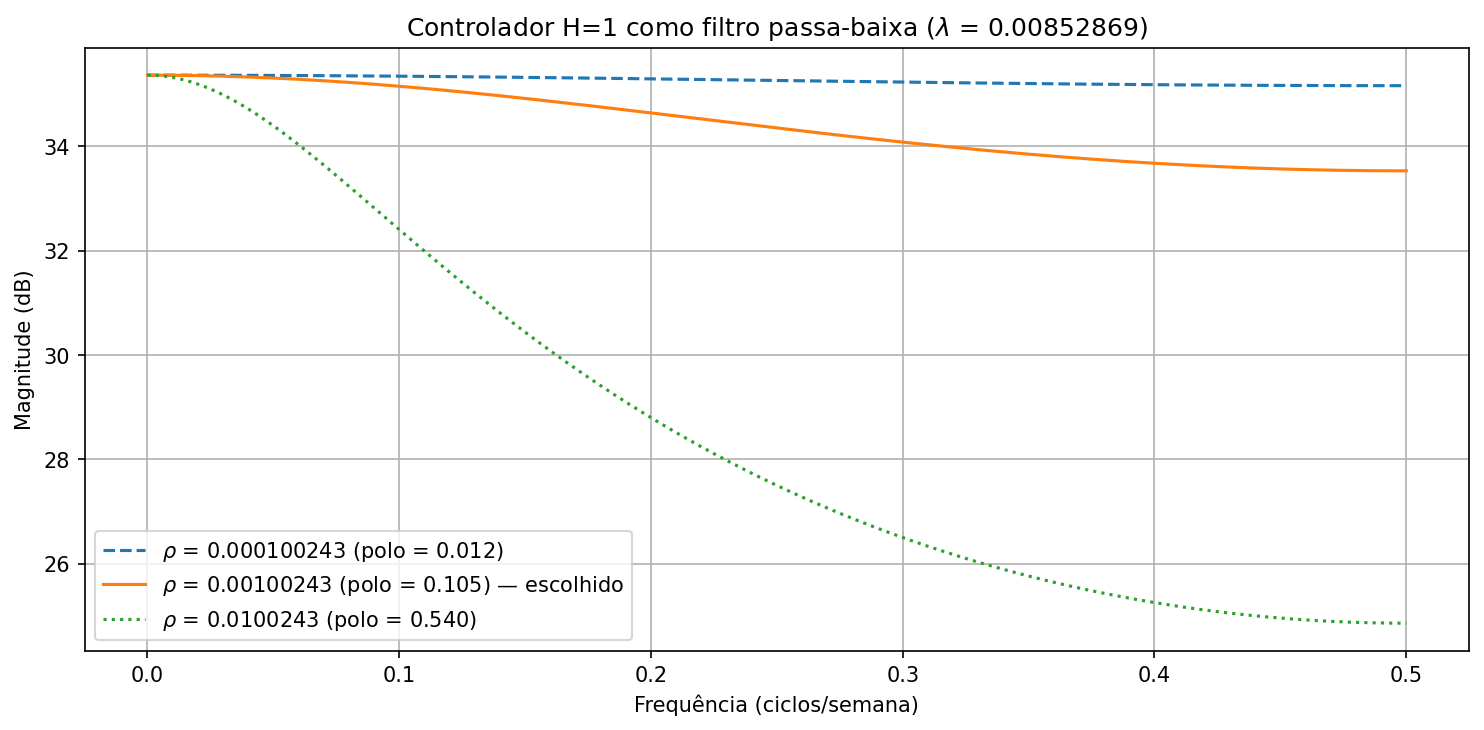
\includegraphics[width=\columnwidth]{figuras/resposta_frequencia_controlador.png}
\caption{Resposta em frequência do controlador $C(z)$ para o $\rho$ selecionado e variações de uma década. Aumentar $\rho$ aproxima o polo de $1$ e estreita a banda do controlador.}
\label{fig:ctrl}
\end{figure}

\subsection{Seleção do horizonte de predição}\label{sec:res-horizonte}

A varredura de $H \in \{1,2,3,4,6,8\}$ na validação produziu Sharpe de $-0{,}884$ para $H=1$ e valores monotonicamente inferiores, saturando em $-0{,}896$ já a partir de $H=3$. O horizonte ótimo é, portanto, unitário --- e com $H^{*}=1$ o MPC coincide exatamente com a lei analítica \eqref{eq:leih1}, coincidência verificada pela suíte de testes; por isso as tabelas seguintes reportam a lei preditiva uma única vez. Este resultado negativo é a confirmação experimental mais direta da análise em $z$: com predição recursiva cujo conteúdo decai como $0{,}55^k$, a predição além de uma ou duas semanas é essencialmente nula, e os termos adicionais do custo \eqref{eq:custompc} apenas somam ruído. A teoria previu o teto; a validação o encontrou.

\subsection{Desempenho no conjunto de teste}\label{sec:res-teste}

A Tabela~\ref{tab:teste} resume o primeiro semestre de 2026, período em que o CDI rendeu $6{,}9\%$. O controlador preditivo obtém Sharpe de $1{,}69$, contra $1{,}08$ do regulador de volatilidade e $0{,}81$ da estratégia passiva. Mais informativo que a ordenação é o padrão de risco: o controle entrega retorno superior ao do ativo ($20{,}4\%$ contra $17{,}6\%$) com metade da volatilidade ($14{,}7\%$ contra $28{,}6\%$) e menos de um terço do rebaixamento máximo ($-4{,}9\%$ contra $-15{,}8\%$), mantendo em média apenas $34\%$ do capital investido. A Fig.~\ref{fig:capital} mostra o mecanismo: a lei dosa a exposição no tempo, participando das altas e recuando nas quedas, em vez de reduzir a exposição uniformemente. O regulador de volatilidade produz redução de risco intermediária sem usar predição alguma (Fig.~\ref{fig:expvol}), e sua variante com viés do ARX fica entre os dois --- coerente com um preditor de valor real, porém modesto.

\begin{table}[!t]
\centering
\caption{Desempenho no conjunto de teste (1º semestre de 2026). $p$ é o valor-$p$ \emph{bootstrap} de não superar o Buy and Hold em Sharpe. O MPC com $H^{*}{=}1$ coincide com o Controle $H{=}1$.}
\label{tab:teste}
\begin{tabular}{lcccccc}
\toprule
Estratégia & Ret.\ (\%) & Sharpe & Vol.\ (\%) & DD (\%) & Pos. & $p$ \\
\midrule
Controle $H{=}1$      & 20,4 & 1,69 & 14,7 & $-4{,}9$  & 0,34 & 0,28 \\
Vol.\ targeting       & 18,5 & 1,08 & 20,9 & $-9{,}1$  & 0,62 & 0,40 \\
Vol.\ targ.\ + ARX    & 17,6 & 1,11 & 18,7 & $-9{,}0$  & 0,62 & 0,23 \\
Buy and Hold          & 17,6 & 0,81 & 28,6 & $-15{,}8$ & 1,00 & ---  \\
\bottomrule
\end{tabular}
\end{table}

\begin{figure}[!t]
\centering
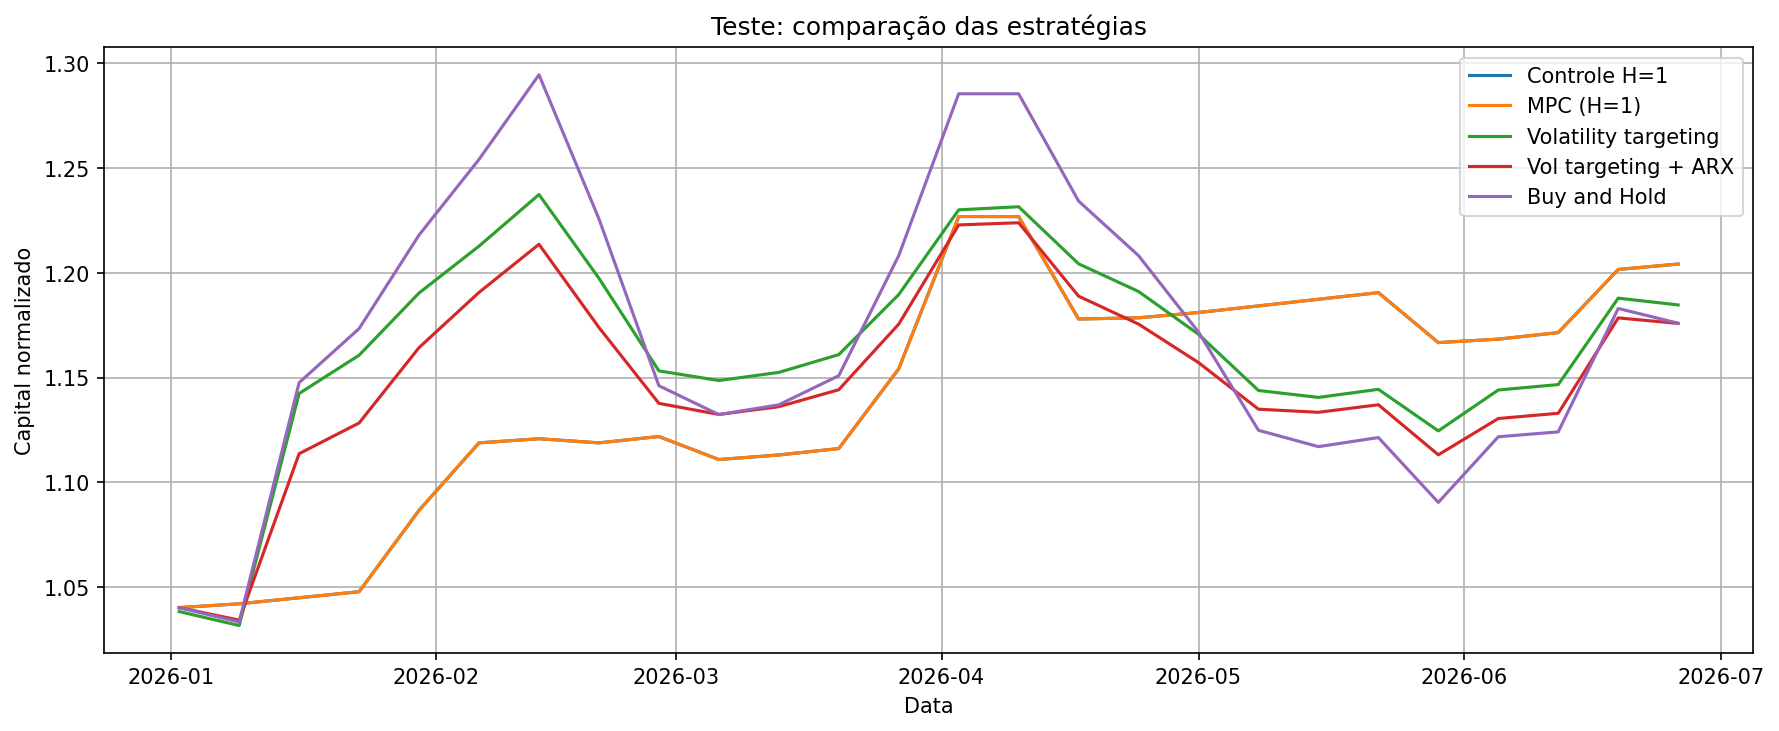
\includegraphics[width=\columnwidth]{figuras/capital_estrategias_teste.png}
\caption{Evolução do capital no conjunto de teste. As leis de controle acompanham a alta do ativo em trajetória mais suave que a estratégia passiva.}
\label{fig:capital}
\end{figure}

\begin{figure}[!t]
\centering
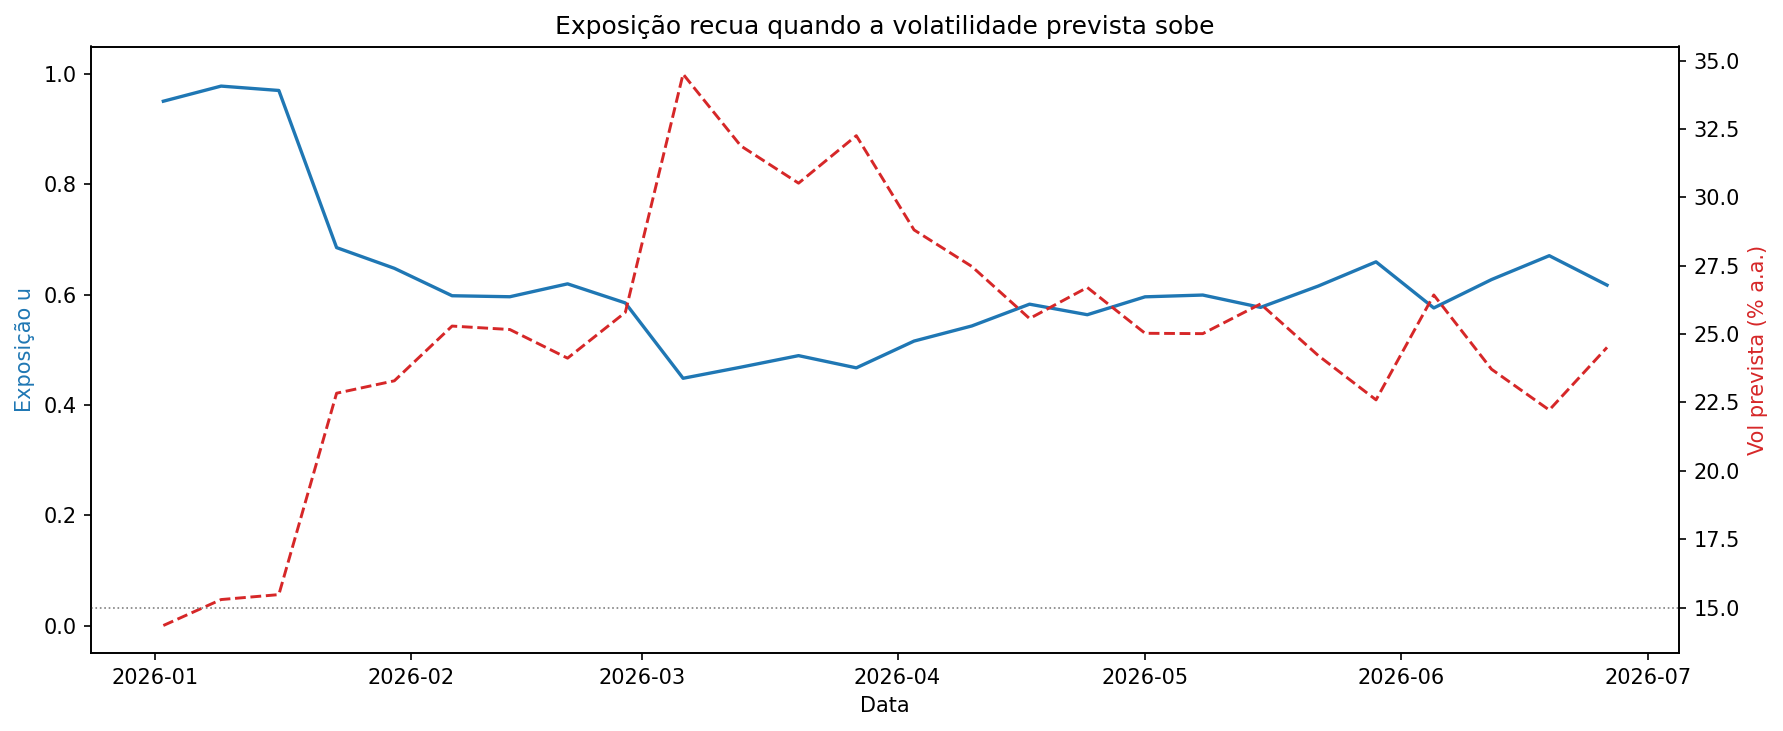
\includegraphics[width=\columnwidth]{figuras/exposicao_vs_volatilidade.png}
\caption{Regulador de volatilidade: a exposição $u[k]$ recua quando a volatilidade prevista pelo filtro EWMA sobe, realimentação sobre a medida de risco.}
\label{fig:expvol}
\end{figure}

\subsection{Validação \emph{walk-forward}}

Uma única janela favorável é evidência fraca; o exercício é repetido de 2025 em diante com re-identificação periódica e sem qualquer informação futura --- inclusive de hiperparâmetros, escolhidos em 2024. A Tabela~\ref{tab:wf} mostra que o padrão persiste e se acentua: Sharpe de $2{,}02$ para o controle preditivo, com volatilidade de $10{,}0\%$ e rebaixamento máximo de $-3{,}1\%$, contra $1{,}52$, $21{,}7\%$ e $-15{,}8\%$ do Buy and Hold. O passivo obteve o maior retorno bruto do período ($93{,}4\%$, contra $64{,}0\%$ do controle, com CDI de $22{,}1\%$), porque a ITSA4 subiu fortemente; o controlador trocou deliberadamente parte do pico de retorno por estabilidade de trajetória, que é exatamente o que as penalizações de esforço e de variação codificam (Fig.~\ref{fig:wf}). O ganho de Sharpe do controle sobre o passivo não atinge significância convencional ($p = 0{,}22$), limitação discutida adiante.

\begin{table}[!t]
\centering
\caption{Validação \emph{walk-forward} (2025 em diante). CDI do período: $22{,}1\%$.}
\label{tab:wf}
\begin{tabular}{lccccc}
\toprule
Estratégia & Ret.\ (\%) & Sharpe & Vol.\ (\%) & DD (\%) & $p$ \\
\midrule
Controle $H{=}1$  & 64,0 & 2,02 & 10,0 & $-3{,}1$  & 0,22 \\
Vol.\ targeting   & 74,0 & 1,54 & 16,2 & $-9{,}1$  & 0,50 \\
Buy and Hold      & 93,4 & 1,52 & 21,7 & $-15{,}8$ & ---  \\
\bottomrule
\end{tabular}
\end{table}

\begin{figure}[!t]
\centering
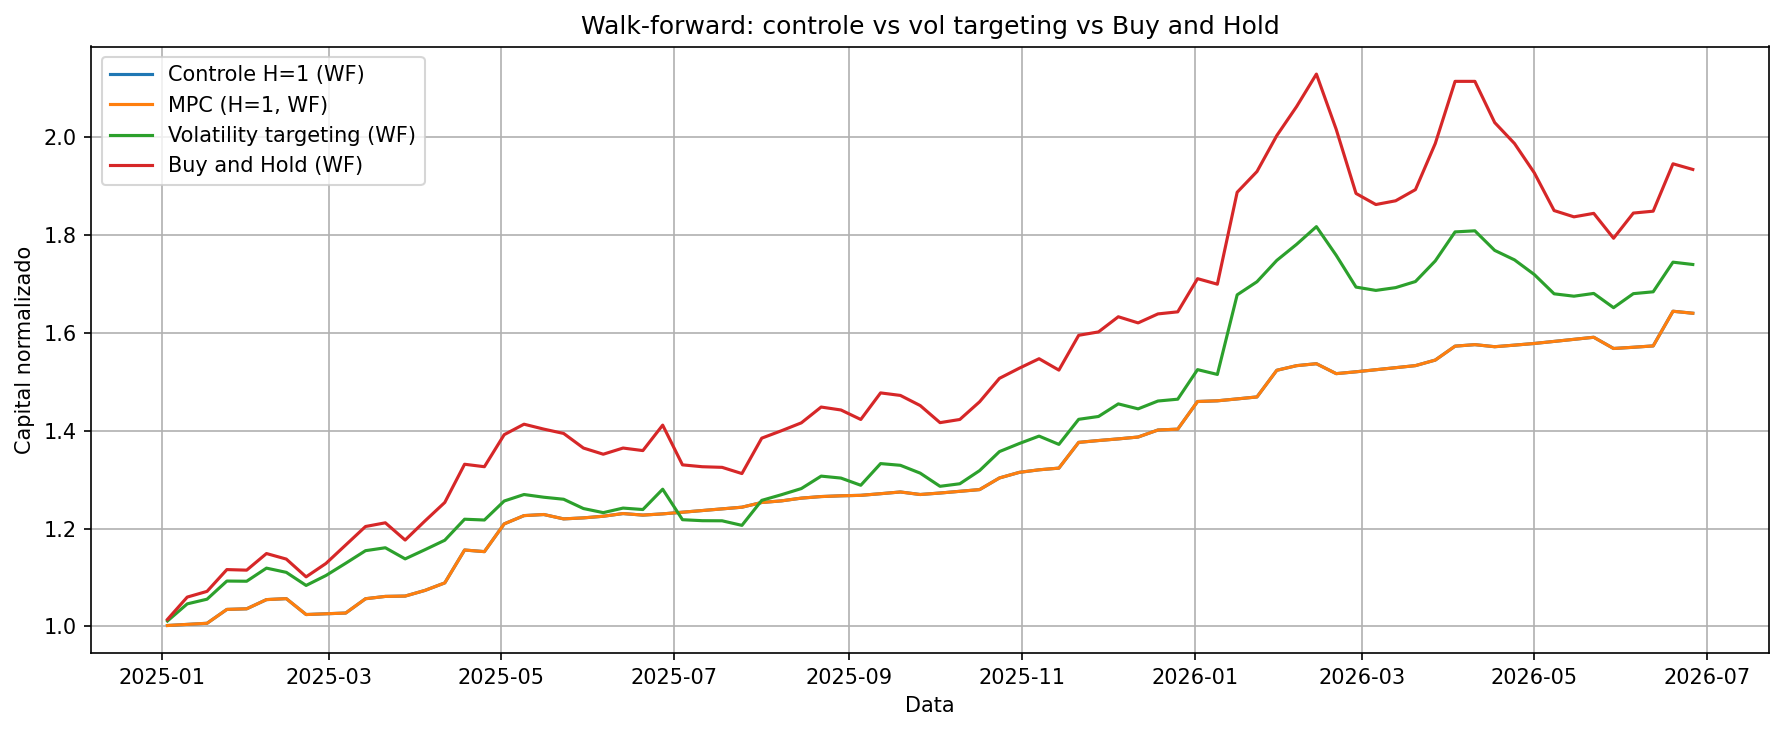
\includegraphics[width=\columnwidth]{figuras/capital_walkforward.png}
\caption{Capital na validação \emph{walk-forward}, com modelo re-identificado apenas com dados passados.}
\label{fig:wf}
\end{figure}

\subsection{Sensibilidade ao custo de transação}

O controlador preditivo gira a carteira ($|\Delta u|$ médio de $0{,}36$ por semana) muito mais que o regulador de volatilidade ($0{,}05$), e o custo entra na planta pelo termo $c\,|\Delta u|$ de \eqref{eq:planta}. A Tabela~\ref{tab:custos} varre $c$ de zero a $0{,}5\%$ por operação: o Sharpe do controle cai de $1{,}82$ para $1{,}16$, mas permanece à frente das alternativas em toda a faixa examinada, enquanto o regulador de volatilidade, quase insensível ao custo, estreita a diferença. A tendência é coerente com a teoria da Seção~\ref{sec:teoria-h1}: com custos maiores, o $\rho$ ótimo cresceria, deslocando o polo do controlador em direção a $1$ e aproximando seu comportamento do regulador lento; a faixa examinada apenas ainda não alcança o ponto de cruzamento.

\begin{table}[!t]
\centering
\caption{Índice de Sharpe no teste em função do custo por operação.}
\label{tab:custos}
\begin{tabular}{lccccc}
\toprule
Estratégia & $c{=}0$ & $0{,}05\%$ & $0{,}1\%$ & $0{,}2\%$ & $0{,}5\%$ \\
\midrule
Controle $H{=}1$   & 1,82 & 1,76 & 1,69 & 1,56 & 1,16 \\
Vol.\ targeting    & 1,10 & 1,09 & 1,08 & 1,07 & 1,01 \\
Vol.\ targ.\ + ARX & 1,15 & 1,13 & 1,11 & 1,07 & 0,95 \\
Buy and Hold       & 0,81 & 0,81 & 0,81 & 0,80 & 0,78 \\
\bottomrule
\end{tabular}
\end{table}

\subsection{Sensibilidade ao atraso}\label{sec:res-atraso}

A Tabela~\ref{tab:atraso} apresenta o experimento da Seção~\ref{sec:teoria-atraso}. Uma semana de atraso reduz o Sharpe do controlador de $1{,}69$ para $0{,}99$ e o retorno de $20{,}4\%$ para $13{,}2\%$; com duas semanas, o desempenho colapsa para próximo de zero. A taxa de degradação é severa porque coincide com a memória do sistema: quando o atraso iguala a profundidade efetiva de $\approx 2$ semanas dos polos, a informação que chega ao controlador já não guarda relação com o estado presente do mercado. O experimento inclui ainda um MPC de horizonte fixo $H=4$, para testar se a predição multipasso mitigaria o atraso por antecipação; a degradação é essencialmente idêntica ($1{,}65 \to 0{,}92 \to 0{,}07$). O resultado negativo tem a mesma raiz estrutural do $H^{*}=1$: a antecipação só compensa atraso se a predição a mais de um passo tiver conteúdo, e o decaimento $0{,}55^k$ o nega. Em termos de projeto, a conclusão prática é direta: nesta malha, investir em reduzir a latência da informação vale mais do que investir em sofisticação do preditor.

\begin{table}[!t]
\centering
\caption{Degradação com atraso de medida de $n$ semanas (teste).}
\label{tab:atraso}
\begin{tabular}{ccccc}
\toprule
 & \multicolumn{2}{c}{Controle $H{=}1$} & \multicolumn{2}{c}{MPC ($H{=}4$)} \\
$n$ & Sharpe & Ret.\ (\%) & Sharpe & Ret.\ (\%) \\
\midrule
0 & 1,69 & 20,4 & 1,65 & 20,0 \\
1 & 0,99 & 13,2 & 0,92 & 12,7 \\
2 & 0,08 & \phantom{0}6,7 & 0,07 & \phantom{0}6,6 \\
\bottomrule
\end{tabular}
\end{table}

\subsection{Discussão}

Os experimentos formam um quadro internamente consistente cuja chave é a constante de tempo do sistema identificado. Os polos de módulo $0{,}55$, robustos à regularização, implicam memória de cerca de duas semanas; dessa única propriedade decorrem o valor modesto porém real do preditor (correlação de $0{,}30$ no \emph{walk-forward}), o horizonte ótimo unitário, a inutilidade da antecipação multipasso contra atraso e a violência da degradação quando o atraso alcança duas semanas. No sentido oposto, a mesma estrutura sustenta o ganho de risco: um preditor fracamente correlacionado com o futuro, aplicado por uma lei que penaliza esforço e variação, basta para entregar o retorno do ativo com metade da volatilidade nas duas janelas de avaliação.

A leitura estatística delimita o alcance das conclusões. Os valores-$p$ de superação do Buy and Hold em Sharpe ($0{,}28$ no teste, $0{,}22$ no \emph{walk-forward}) não atingem significância convencional, o que era esperado: janelas de 26 e 78 semanas têm baixo poder para discriminar índices de Sharpe. A afirmação que os dados sustentam com folga não é ``o controle rende mais'', e sim ``o controle rende de forma comparável com risco muito menor'' --- a redução de volatilidade e de rebaixamento é consistente nas duas janelas, em toda a faixa de custos examinada e nos dois reguladores (preditivo e de volatilidade), que operam por mecanismos independentes. Registre-se, por fim, que a janela de avaliação coincidiu com um período de alta do ativo, o que favorece qualquer estratégia comprada; nada garante desempenho semelhante em regimes de queda prolongada, cenário em que a exposição parcial do controle tenderia, por construção, a limitar perdas, mas para o qual não há evidência experimental aqui.

\section{Conclusão}\label{sec:conclusao}

Este trabalho tratou a alocação dinâmica em ITSA4 como um problema de controle em tempo discreto e percorreu o ciclo completo de projeto: identificação ARX, caracterização por função de transferência, síntese de leis de controle por otimização numérica com refino de Nelder--Mead, e avaliação fora da amostra com testes de significância e análises de sensibilidade. A contribuição central é metodológica e interpretativa: mostrar que a posição dos polos do sistema identificado --- estável, com raio espectral de $0{,}55$ robusto à regularização --- funciona como variável explicativa unificadora dos resultados, prevendo o horizonte de predição ótimo unitário, a tolerância a atraso de no máximo uma semana e o teto de valor do preditor, todos confirmados experimentalmente.

Do ponto de vista de desempenho, as leis de controle entregaram o retorno do ativo com aproximadamente metade da volatilidade e um terço do rebaixamento máximo, no teste e na validação \emph{walk-forward}, com robustez a custos de transação até $0{,}5\%$ por operação; a vantagem em retorno sobre a estratégia passiva, contudo, não é estatisticamente significativa nas janelas disponíveis, e a conclusão defensável restringe-se à gestão de risco. As limitações principais são o tamanho das janelas fora da amostra, o uso de um único ativo e um período de avaliação em alta. Como trabalhos futuros, destacam-se a reescolha dos hiperparâmetros dentro de cada janela do \emph{walk-forward}, a identificação variante no tempo por filtro de Kalman --- extensão natural da filtragem de primeira ordem aqui empregada --- e uma formulação de controle preditivo que incorpore explicitamente a incerteza da predição no custo.

\appendices
\section{Manual do Usuário}\label{ap:manual}

O projeto requer Python~3 e as dependências fixadas em \texttt{requirements.txt} (numpy, pandas, matplotlib, scikit-learn, scipy, yfinance e requests). A partir da pasta raiz:
\begin{verbatim}
python -m venv .venv
.venv\Scripts\activate    (Windows)
pip install -r requirements.txt
\end{verbatim}
A suíte de verificação roda offline, sobre dados sintéticos, e confere as peças centrais do projeto (resolvedor do programa quadrático, equivalências do controlador de horizonte unitário, banda dos filtros de primeira ordem, confinamento do refino de Nelder--Mead, ausência de vazamento temporal e degradação sob atraso):
\begin{verbatim}
py tests\test_projeto.py
\end{verbatim}
O experimento completo é executado por:
\begin{verbatim}
py main.py
\end{verbatim}
Na primeira execução, as séries de mercado (Yahoo Finance) e do CDI (SGS/BCB) são baixadas e salvas em \texttt{outputs/snapshot/}, o que exige internet; execuções seguintes recarregam o \emph{snapshot}, tornando os resultados reprodutíveis --- para forçar novo download, basta apagar essa pasta. As tabelas em CSV (qualidade do preditor, hiperparâmetros, seleção de horizonte, filtros, resumos de teste e \emph{walk-forward}, sensibilidades a custo, atraso e regularização) são gravadas em \texttt{outputs/}, e as figuras em \texttt{figuras/}, pasta referenciada por este documento. Os parâmetros do estudo concentram-se em \texttt{src/config.py}.

\begin{thebibliography}{18}
\bibitem{fama1970} E.~F. Fama, ``Efficient capital markets: A review of theory and empirical work,'' \emph{The Journal of Finance}, vol.~25, no.~2, pp.~383--417, 1970.
\bibitem{ljung1999} L.~Ljung, \emph{System Identification: Theory for the User}, 2nd~ed. Upper Saddle River, NJ: Prentice-Hall, 1999.
\bibitem{hoerl1970} A.~E. Hoerl and R.~W. Kennard, ``Ridge regression: Biased estimation for nonorthogonal problems,'' \emph{Technometrics}, vol.~12, no.~1, pp.~55--67, 1970.
\bibitem{astrom1997} K.~J. \r{A}str\"om and B.~Wittenmark, \emph{Computer-Controlled Systems: Theory and Design}, 3rd~ed. Upper Saddle River, NJ: Prentice-Hall, 1997.
\bibitem{anderson1990} B.~D.~O. Anderson and J.~B. Moore, \emph{Optimal Control: Linear Quadratic Methods}. Englewood Cliffs, NJ: Prentice-Hall, 1990.
\bibitem{camacho2007} E.~F. Camacho and C.~Bordons, \emph{Model Predictive Control}, 2nd~ed. London, U.K.: Springer, 2007.
\bibitem{mayne2000} D.~Q. Mayne, J.~B. Rawlings, C.~V. Rao, and P.~O.~M. Scokaert, ``Constrained model predictive control: Stability and optimality,'' \emph{Automatica}, vol.~36, no.~6, pp.~789--814, 2000.
\bibitem{boyd2004} S.~Boyd and L.~Vandenberghe, \emph{Convex Optimization}. Cambridge, U.K.: Cambridge Univ. Press, 2004.
\bibitem{nelder1965} J.~A. Nelder and R.~Mead, ``A simplex method for function minimization,'' \emph{The Computer Journal}, vol.~7, no.~4, pp.~308--313, 1965.
\bibitem{engle1982} R.~F. Engle, ``Autoregressive conditional heteroscedasticity with estimates of the variance of United Kingdom inflation,'' \emph{Econometrica}, vol.~50, no.~4, pp.~987--1007, 1982.
\bibitem{bollerslev1986} T.~Bollerslev, ``Generalized autoregressive conditional heteroskedasticity,'' \emph{Journal of Econometrics}, vol.~31, no.~3, pp.~307--327, 1986.
\bibitem{cont2001} R.~Cont, ``Empirical properties of asset returns: Stylized facts and statistical issues,'' \emph{Quantitative Finance}, vol.~1, no.~2, pp.~223--236, 2001.
\bibitem{riskmetrics1996} J.P.~Morgan/Reuters, \emph{RiskMetrics: Technical Document}, 4th~ed. New York: J.P.~Morgan, 1996.
\bibitem{moreira2017} A.~Moreira and T.~Muir, ``Volatility-managed portfolios,'' \emph{The Journal of Finance}, vol.~72, no.~4, pp.~1611--1644, 2017.
\bibitem{sharpe1994} W.~F. Sharpe, ``The Sharpe ratio,'' \emph{The Journal of Portfolio Management}, vol.~21, no.~1, pp.~49--58, 1994.
\bibitem{kunsch1989} H.~R. K\"unsch, ``The jackknife and the bootstrap for general stationary observations,'' \emph{The Annals of Statistics}, vol.~17, no.~3, pp.~1217--1241, 1989.
\bibitem{pedregosa2011} F.~Pedregosa \emph{et al.}, ``Scikit-learn: Machine learning in Python,'' \emph{Journal of Machine Learning Research}, vol.~12, pp.~2825--2830, 2011.
\bibitem{virtanen2020} P.~Virtanen \emph{et al.}, ``SciPy 1.0: Fundamental algorithms for scientific computing in Python,'' \emph{Nature Methods}, vol.~17, no.~3, pp.~261--272, 2020.
\end{thebibliography}

\end{document}
